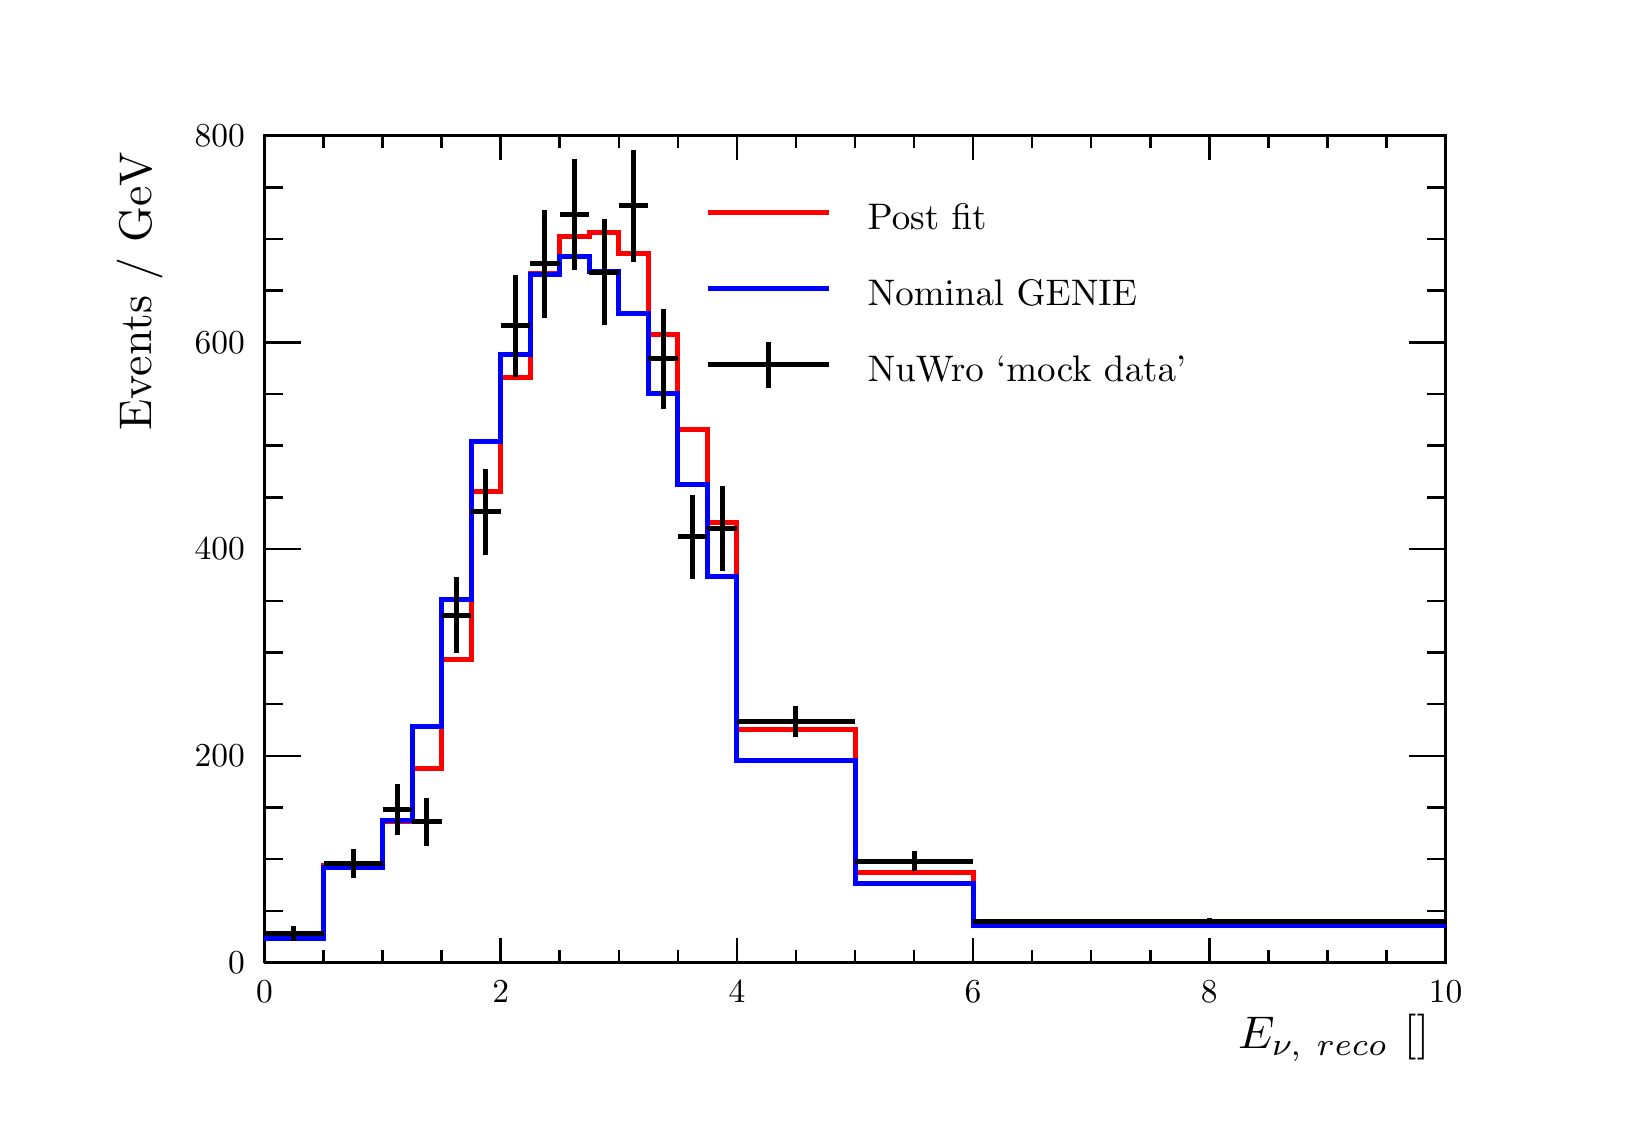
\begin{tikzpicture}
\pgfdeclareplotmark{cross} {
\pgfpathmoveto{\pgfpoint{-0.3\pgfplotmarksize}{\pgfplotmarksize}}
\pgfpathlineto{\pgfpoint{+0.3\pgfplotmarksize}{\pgfplotmarksize}}
\pgfpathlineto{\pgfpoint{+0.3\pgfplotmarksize}{0.3\pgfplotmarksize}}
\pgfpathlineto{\pgfpoint{+1\pgfplotmarksize}{0.3\pgfplotmarksize}}
\pgfpathlineto{\pgfpoint{+1\pgfplotmarksize}{-0.3\pgfplotmarksize}}
\pgfpathlineto{\pgfpoint{+0.3\pgfplotmarksize}{-0.3\pgfplotmarksize}}
\pgfpathlineto{\pgfpoint{+0.3\pgfplotmarksize}{-1.\pgfplotmarksize}}
\pgfpathlineto{\pgfpoint{-0.3\pgfplotmarksize}{-1.\pgfplotmarksize}}
\pgfpathlineto{\pgfpoint{-0.3\pgfplotmarksize}{-0.3\pgfplotmarksize}}
\pgfpathlineto{\pgfpoint{-1.\pgfplotmarksize}{-0.3\pgfplotmarksize}}
\pgfpathlineto{\pgfpoint{-1.\pgfplotmarksize}{0.3\pgfplotmarksize}}
\pgfpathlineto{\pgfpoint{-0.3\pgfplotmarksize}{0.3\pgfplotmarksize}}
\pgfpathclose
\pgfusepathqstroke
}
\pgfdeclareplotmark{cross*} {
\pgfpathmoveto{\pgfpoint{-0.3\pgfplotmarksize}{\pgfplotmarksize}}
\pgfpathlineto{\pgfpoint{+0.3\pgfplotmarksize}{\pgfplotmarksize}}
\pgfpathlineto{\pgfpoint{+0.3\pgfplotmarksize}{0.3\pgfplotmarksize}}
\pgfpathlineto{\pgfpoint{+1\pgfplotmarksize}{0.3\pgfplotmarksize}}
\pgfpathlineto{\pgfpoint{+1\pgfplotmarksize}{-0.3\pgfplotmarksize}}
\pgfpathlineto{\pgfpoint{+0.3\pgfplotmarksize}{-0.3\pgfplotmarksize}}
\pgfpathlineto{\pgfpoint{+0.3\pgfplotmarksize}{-1.\pgfplotmarksize}}
\pgfpathlineto{\pgfpoint{-0.3\pgfplotmarksize}{-1.\pgfplotmarksize}}
\pgfpathlineto{\pgfpoint{-0.3\pgfplotmarksize}{-0.3\pgfplotmarksize}}
\pgfpathlineto{\pgfpoint{-1.\pgfplotmarksize}{-0.3\pgfplotmarksize}}
\pgfpathlineto{\pgfpoint{-1.\pgfplotmarksize}{0.3\pgfplotmarksize}}
\pgfpathlineto{\pgfpoint{-0.3\pgfplotmarksize}{0.3\pgfplotmarksize}}
\pgfpathclose
\pgfusepathqfillstroke
}
\pgfdeclareplotmark{newstar} {
\pgfpathmoveto{\pgfqpoint{0pt}{\pgfplotmarksize}}
\pgfpathlineto{\pgfqpointpolar{44}{0.5\pgfplotmarksize}}
\pgfpathlineto{\pgfqpointpolar{18}{\pgfplotmarksize}}
\pgfpathlineto{\pgfqpointpolar{-20}{0.5\pgfplotmarksize}}
\pgfpathlineto{\pgfqpointpolar{-54}{\pgfplotmarksize}}
\pgfpathlineto{\pgfqpointpolar{-90}{0.5\pgfplotmarksize}}
\pgfpathlineto{\pgfqpointpolar{234}{\pgfplotmarksize}}
\pgfpathlineto{\pgfqpointpolar{198}{0.5\pgfplotmarksize}}
\pgfpathlineto{\pgfqpointpolar{162}{\pgfplotmarksize}}
\pgfpathlineto{\pgfqpointpolar{134}{0.5\pgfplotmarksize}}
\pgfpathclose
\pgfusepathqstroke
}
\pgfdeclareplotmark{newstar*} {
\pgfpathmoveto{\pgfqpoint{0pt}{\pgfplotmarksize}}
\pgfpathlineto{\pgfqpointpolar{44}{0.5\pgfplotmarksize}}
\pgfpathlineto{\pgfqpointpolar{18}{\pgfplotmarksize}}
\pgfpathlineto{\pgfqpointpolar{-20}{0.5\pgfplotmarksize}}
\pgfpathlineto{\pgfqpointpolar{-54}{\pgfplotmarksize}}
\pgfpathlineto{\pgfqpointpolar{-90}{0.5\pgfplotmarksize}}
\pgfpathlineto{\pgfqpointpolar{234}{\pgfplotmarksize}}
\pgfpathlineto{\pgfqpointpolar{198}{0.5\pgfplotmarksize}}
\pgfpathlineto{\pgfqpointpolar{162}{\pgfplotmarksize}}
\pgfpathlineto{\pgfqpointpolar{134}{0.5\pgfplotmarksize}}
\pgfpathclose
\pgfusepathqfillstroke
}
\definecolor{c}{rgb}{1,1,1};
\draw [color=c, fill=c] (0,0) rectangle (20,13.639);
\draw [color=c, fill=c] (3,1.77307) rectangle (18,12.2751);
\definecolor{c}{rgb}{0,0,0};
\draw [c,line width=0.9] (3,1.77307) -- (3,12.2751) -- (18,12.2751) -- (18,1.77307) -- (3,1.77307);
\definecolor{c}{rgb}{1,1,1};
\draw [color=c, fill=c] (3,1.77307) rectangle (18,12.2751);
\definecolor{c}{rgb}{0,0,0};
\draw [c,line width=0.9] (3,1.77307) -- (3,12.2751) -- (18,12.2751) -- (18,1.77307) -- (3,1.77307);
\definecolor{c}{rgb}{1,0,0};
\draw [c,line width=1.8] (3,2.09451) -- (3.75,2.09451) -- (3.75,3.0091) -- (4.5,3.0091) -- (4.5,3.56676) -- (4.875,3.56676) -- (4.875,4.23968) -- (5.25,4.23968) -- (5.25,5.62292) -- (5.625,5.62292) -- (5.625,7.75072) -- (6,7.75072) -- (6,9.20668) --
 (6.375,9.20668) -- (6.375,10.519) -- (6.75,10.519) -- (6.75,10.9918) -- (7.125,10.9918) -- (7.125,11.0498) -- (7.5,11.0498) -- (7.5,10.7751) -- (7.875,10.7751) -- (7.875,9.74937) -- (8.25,9.74937) -- (8.25,8.53776) -- (8.625,8.53776) --
 (8.625,7.3619) -- (9,7.3619) -- (9,4.7316) -- (10.5,4.7316) -- (10.5,2.91667) -- (12,2.91667) -- (12,2.29467) -- (18,2.29467);
\definecolor{c}{rgb}{0,0,0};
\draw [c,line width=0.9] (3,1.77307) -- (18,1.77307);
\draw [c,line width=0.9] (3,2.07994) -- (3,1.77307);
\draw [c,line width=0.9] (3.75,1.9265) -- (3.75,1.77307);
\draw [c,line width=0.9] (4.5,1.9265) -- (4.5,1.77307);
\draw [c,line width=0.9] (5.25,1.9265) -- (5.25,1.77307);
\draw [c,line width=0.9] (6,2.07994) -- (6,1.77307);
\draw [c,line width=0.9] (6.75,1.9265) -- (6.75,1.77307);
\draw [c,line width=0.9] (7.5,1.9265) -- (7.5,1.77307);
\draw [c,line width=0.9] (8.25,1.9265) -- (8.25,1.77307);
\draw [c,line width=0.9] (9,2.07994) -- (9,1.77307);
\draw [c,line width=0.9] (9.75,1.9265) -- (9.75,1.77307);
\draw [c,line width=0.9] (10.5,1.9265) -- (10.5,1.77307);
\draw [c,line width=0.9] (11.25,1.9265) -- (11.25,1.77307);
\draw [c,line width=0.9] (12,2.07994) -- (12,1.77307);
\draw [c,line width=0.9] (12.75,1.9265) -- (12.75,1.77307);
\draw [c,line width=0.9] (13.5,1.9265) -- (13.5,1.77307);
\draw [c,line width=0.9] (14.25,1.9265) -- (14.25,1.77307);
\draw [c,line width=0.9] (15,2.07994) -- (15,1.77307);
\draw [c,line width=0.9] (15.75,1.9265) -- (15.75,1.77307);
\draw [c,line width=0.9] (16.5,1.9265) -- (16.5,1.77307);
\draw [c,line width=0.9] (17.25,1.9265) -- (17.25,1.77307);
\draw [c,line width=0.9] (18,2.07994) -- (18,1.77307);
\draw [anchor=base] (3,1.26842) node[scale=1.20912, color=c, rotate=0]{0};
\draw [anchor=base] (6,1.26842) node[scale=1.20912, color=c, rotate=0]{2};
\draw [anchor=base] (9,1.26842) node[scale=1.20912, color=c, rotate=0]{4};
\draw [anchor=base] (12,1.26842) node[scale=1.20912, color=c, rotate=0]{6};
\draw [anchor=base] (15,1.26842) node[scale=1.20912, color=c, rotate=0]{8};
\draw [anchor=base] (18,1.26842) node[scale=1.20912, color=c, rotate=0]{10};
\draw [anchor= east] (18,0.812882) node[scale=1.65459, color=c, rotate=0]{$E_{\nu,~\text{reco}}$ [\si{\GeV}]};
\draw [c,line width=0.9] (3,12.2751) -- (18,12.2751);
\draw [c,line width=0.9] (3,11.9682) -- (3,12.2751);
\draw [c,line width=0.9] (3.75,12.1216) -- (3.75,12.2751);
\draw [c,line width=0.9] (4.5,12.1216) -- (4.5,12.2751);
\draw [c,line width=0.9] (5.25,12.1216) -- (5.25,12.2751);
\draw [c,line width=0.9] (6,11.9682) -- (6,12.2751);
\draw [c,line width=0.9] (6.75,12.1216) -- (6.75,12.2751);
\draw [c,line width=0.9] (7.5,12.1216) -- (7.5,12.2751);
\draw [c,line width=0.9] (8.25,12.1216) -- (8.25,12.2751);
\draw [c,line width=0.9] (9,11.9682) -- (9,12.2751);
\draw [c,line width=0.9] (9.75,12.1216) -- (9.75,12.2751);
\draw [c,line width=0.9] (10.5,12.1216) -- (10.5,12.2751);
\draw [c,line width=0.9] (11.25,12.1216) -- (11.25,12.2751);
\draw [c,line width=0.9] (12,11.9682) -- (12,12.2751);
\draw [c,line width=0.9] (12.75,12.1216) -- (12.75,12.2751);
\draw [c,line width=0.9] (13.5,12.1216) -- (13.5,12.2751);
\draw [c,line width=0.9] (14.25,12.1216) -- (14.25,12.2751);
\draw [c,line width=0.9] (15,11.9682) -- (15,12.2751);
\draw [c,line width=0.9] (15.75,12.1216) -- (15.75,12.2751);
\draw [c,line width=0.9] (16.5,12.1216) -- (16.5,12.2751);
\draw [c,line width=0.9] (17.25,12.1216) -- (17.25,12.2751);
\draw [c,line width=0.9] (18,11.9682) -- (18,12.2751);
\draw [c,line width=0.9] (3,1.77307) -- (3,12.2751);
\draw [c,line width=0.9] (3.462,1.77307) -- (3,1.77307);
\draw [c,line width=0.9] (3.231,2.42944) -- (3,2.42944);
\draw [c,line width=0.9] (3.231,3.08582) -- (3,3.08582);
\draw [c,line width=0.9] (3.231,3.74219) -- (3,3.74219);
\draw [c,line width=0.9] (3.462,4.39857) -- (3,4.39857);
\draw [c,line width=0.9] (3.231,5.05494) -- (3,5.05494);
\draw [c,line width=0.9] (3.231,5.71132) -- (3,5.71132);
\draw [c,line width=0.9] (3.231,6.36769) -- (3,6.36769);
\draw [c,line width=0.9] (3.462,7.02407) -- (3,7.02407);
\draw [c,line width=0.9] (3.231,7.68044) -- (3,7.68044);
\draw [c,line width=0.9] (3.231,8.33682) -- (3,8.33682);
\draw [c,line width=0.9] (3.231,8.99319) -- (3,8.99319);
\draw [c,line width=0.9] (3.462,9.64957) -- (3,9.64957);
\draw [c,line width=0.9] (3.231,10.3059) -- (3,10.3059);
\draw [c,line width=0.9] (3.231,10.9623) -- (3,10.9623);
\draw [c,line width=0.9] (3.231,11.6187) -- (3,11.6187);
\draw [c,line width=0.9] (3.462,12.2751) -- (3,12.2751);
\draw [anchor= east] (2.9,1.77307) node[scale=1.20912, color=c, rotate=0]{0};
\draw [anchor= east] (2.9,4.39857) node[scale=1.20912, color=c, rotate=0]{200};
\draw [anchor= east] (2.9,7.02407) node[scale=1.20912, color=c, rotate=0]{400};
\draw [anchor= east] (2.9,9.64957) node[scale=1.20912, color=c, rotate=0]{600};
\draw [anchor= east] (2.9,12.2751) node[scale=1.20912, color=c, rotate=0]{800};
\draw [anchor= east] (1.416,12.2751) node[scale=1.65459, color=c, rotate=90]{Events / GeV};
\draw [c,line width=0.9] (18,1.77307) -- (18,12.2751);
\draw [c,line width=0.9] (17.538,1.77307) -- (18,1.77307);
\draw [c,line width=0.9] (17.769,2.42944) -- (18,2.42944);
\draw [c,line width=0.9] (17.769,3.08582) -- (18,3.08582);
\draw [c,line width=0.9] (17.769,3.74219) -- (18,3.74219);
\draw [c,line width=0.9] (17.538,4.39857) -- (18,4.39857);
\draw [c,line width=0.9] (17.769,5.05494) -- (18,5.05494);
\draw [c,line width=0.9] (17.769,5.71132) -- (18,5.71132);
\draw [c,line width=0.9] (17.769,6.36769) -- (18,6.36769);
\draw [c,line width=0.9] (17.538,7.02407) -- (18,7.02407);
\draw [c,line width=0.9] (17.769,7.68044) -- (18,7.68044);
\draw [c,line width=0.9] (17.769,8.33682) -- (18,8.33682);
\draw [c,line width=0.9] (17.769,8.99319) -- (18,8.99319);
\draw [c,line width=0.9] (17.538,9.64957) -- (18,9.64957);
\draw [c,line width=0.9] (17.769,10.3059) -- (18,10.3059);
\draw [c,line width=0.9] (17.769,10.9623) -- (18,10.9623);
\draw [c,line width=0.9] (17.769,11.6187) -- (18,11.6187);
\draw [c,line width=0.9] (17.538,12.2751) -- (18,12.2751);
\definecolor{c}{rgb}{0,0,1};
\draw [c,line width=1.8] (3,2.07411) -- (3.75,2.07411) -- (3.75,2.98588) -- (4.5,2.98588) -- (4.5,3.57979) -- (4.875,3.57979) -- (4.875,4.77283) -- (5.25,4.77283) -- (5.25,6.38982) -- (5.625,6.38982) -- (5.625,8.39274) -- (6,8.39274) -- (6,9.49943)
 -- (6.375,9.49943) -- (6.375,10.5103) -- (6.75,10.5103) -- (6.75,10.7386) -- (7.125,10.7386) -- (7.125,10.5487) -- (7.5,10.5487) -- (7.5,10.0216) -- (7.875,10.0216) -- (7.875,8.99521) -- (8.25,8.99521) -- (8.25,7.84697) -- (8.625,7.84697) --
 (8.625,6.67145) -- (9,6.67145) -- (9,4.34009) -- (10.5,4.34009) -- (10.5,2.77518) -- (12,2.77518) -- (12,2.24504) -- (18,2.24504);
\definecolor{c}{rgb}{0,0,0};
\draw [c,line width=1.8] (3.375,2.0424) -- (3.375,2.14064);
\draw [c,line width=1.8] (3.375,2.14064) -- (3.375,2.23887);
\draw [c,line width=1.8] (3,2.14064) -- (3.375,2.14064);
\draw [c,line width=1.8] (3.375,2.14064) -- (3.75,2.14064);
\foreach \P in {(3.375,2.14064)}{\draw[mark options={color=c,fill=c},mark size=2.402402pt, line width=0.000000pt, mark=*,mark size=1pt] plot coordinates {\P};}
\draw [c,line width=1.8] (4.125,2.85141) -- (4.125,3.03331);
\draw [c,line width=1.8] (4.125,3.03331) -- (4.125,3.21521);
\draw [c,line width=1.8] (3.75,3.03331) -- (4.125,3.03331);
\draw [c,line width=1.8] (4.125,3.03331) -- (4.5,3.03331);
\foreach \P in {(4.125,3.03331)}{\draw[mark options={color=c,fill=c},mark size=2.402402pt, line width=0.000000pt, mark=*,mark size=1pt] plot coordinates {\P};}
\draw [c,line width=1.8] (4.6875,3.39653) -- (4.6875,3.71594);
\draw [c,line width=1.8] (4.6875,3.71594) -- (4.6875,4.03534);
\draw [c,line width=1.8] (4.5,3.71594) -- (4.6875,3.71594);
\draw [c,line width=1.8] (4.6875,3.71594) -- (4.875,3.71594);
\foreach \P in {(4.6875,3.71594)}{\draw[mark options={color=c,fill=c},mark size=2.402402pt, line width=0.000000pt, mark=*,mark size=1pt] plot coordinates {\P};}
\draw [c,line width=1.8] (5.0625,3.25222) -- (5.0625,3.55841);
\draw [c,line width=1.8] (5.0625,3.55841) -- (5.0625,3.86459);
\draw [c,line width=1.8] (4.875,3.55841) -- (5.0625,3.55841);
\draw [c,line width=1.8] (5.0625,3.55841) -- (5.25,3.55841);
\foreach \P in {(5.0625,3.55841)}{\draw[mark options={color=c,fill=c},mark size=2.402402pt, line width=0.000000pt, mark=*,mark size=1pt] plot coordinates {\P};}
\draw [c,line width=1.8] (5.4375,5.70265) -- (5.4375,6.18391);
\draw [c,line width=1.8] (5.4375,6.18391) -- (5.4375,6.66517);
\draw [c,line width=1.8] (5.25,6.18391) -- (5.4375,6.18391);
\draw [c,line width=1.8] (5.4375,6.18391) -- (5.625,6.18391);
\foreach \P in {(5.4375,6.18391)}{\draw[mark options={color=c,fill=c},mark size=2.402402pt, line width=0.000000pt, mark=*,mark size=1pt] plot coordinates {\P};}
\draw [c,line width=1.8] (5.8125,6.94844) -- (5.8125,7.49666);
\draw [c,line width=1.8] (5.8125,7.49666) -- (5.8125,8.04488);
\draw [c,line width=1.8] (5.625,7.49666) -- (5.8125,7.49666);
\draw [c,line width=1.8] (5.8125,7.49666) -- (6,7.49666);
\foreach \P in {(5.8125,7.49666)}{\draw[mark options={color=c,fill=c},mark size=2.402402pt, line width=0.000000pt, mark=*,mark size=1pt] plot coordinates {\P};}
\draw [c,line width=1.8] (6.1875,9.20798) -- (6.1875,9.85961);
\draw [c,line width=1.8] (6.1875,9.85961) -- (6.1875,10.5112);
\draw [c,line width=1.8] (6,9.85961) -- (6.1875,9.85961);
\draw [c,line width=1.8] (6.1875,9.85961) -- (6.375,9.85961);
\foreach \P in {(6.1875,9.85961)}{\draw[mark options={color=c,fill=c},mark size=2.402402pt, line width=0.000000pt, mark=*,mark size=1pt] plot coordinates {\P};}
\draw [c,line width=1.8] (6.5625,9.96463) -- (6.5625,10.6473);
\draw [c,line width=1.8] (6.5625,10.6473) -- (6.5625,11.3299);
\draw [c,line width=1.8] (6.375,10.6473) -- (6.5625,10.6473);
\draw [c,line width=1.8] (6.5625,10.6473) -- (6.75,10.6473);
\foreach \P in {(6.5625,10.6473)}{\draw[mark options={color=c,fill=c},mark size=2.402402pt, line width=0.000000pt, mark=*,mark size=1pt] plot coordinates {\P};}
\draw [c,line width=1.8] (6.9375,10.5709) -- (6.9375,11.2774);
\draw [c,line width=1.8] (6.9375,11.2774) -- (6.9375,11.9838);
\draw [c,line width=1.8] (6.75,11.2774) -- (6.9375,11.2774);
\draw [c,line width=1.8] (6.9375,11.2774) -- (7.125,11.2774);
\foreach \P in {(6.9375,11.2774)}{\draw[mark options={color=c,fill=c},mark size=2.402402pt, line width=0.000000pt, mark=*,mark size=1pt] plot coordinates {\P};}
\draw [c,line width=1.8] (7.3125,9.86366) -- (7.3125,10.5422);
\draw [c,line width=1.8] (7.3125,10.5422) -- (7.3125,11.2208);
\draw [c,line width=1.8] (7.125,10.5422) -- (7.3125,10.5422);
\draw [c,line width=1.8] (7.3125,10.5422) -- (7.5,10.5422);
\foreach \P in {(7.3125,10.5422)}{\draw[mark options={color=c,fill=c},mark size=2.402402pt, line width=0.000000pt, mark=*,mark size=1pt] plot coordinates {\P};}
\draw [c,line width=1.8] (7.6875,10.6721) -- (7.6875,11.3824);
\draw [c,line width=1.8] (7.6875,11.3824) -- (7.6875,12.0927);
\draw [c,line width=1.8] (7.5,11.3824) -- (7.6875,11.3824);
\draw [c,line width=1.8] (7.6875,11.3824) -- (7.875,11.3824);
\foreach \P in {(7.6875,11.3824)}{\draw[mark options={color=c,fill=c},mark size=2.402402pt, line width=0.000000pt, mark=*,mark size=1pt] plot coordinates {\P};}
\draw [c,line width=1.8] (8.0625,8.80505) -- (8.0625,9.43953);
\draw [c,line width=1.8] (8.0625,9.43953) -- (8.0625,10.074);
\draw [c,line width=1.8] (7.875,9.43953) -- (8.0625,9.43953);
\draw [c,line width=1.8] (8.0625,9.43953) -- (8.25,9.43953);
\foreach \P in {(8.0625,9.43953)}{\draw[mark options={color=c,fill=c},mark size=2.402402pt, line width=0.000000pt, mark=*,mark size=1pt] plot coordinates {\P};}
\draw [c,line width=1.8] (8.4375,6.64868) -- (8.4375,7.1816);
\draw [c,line width=1.8] (8.4375,7.1816) -- (8.4375,7.71452);
\draw [c,line width=1.8] (8.25,7.1816) -- (8.4375,7.1816);
\draw [c,line width=1.8] (8.4375,7.1816) -- (8.625,7.1816);
\foreach \P in {(8.4375,7.1816)}{\draw[mark options={color=c,fill=c},mark size=2.402402pt, line width=0.000000pt, mark=*,mark size=1pt] plot coordinates {\P};}
\draw [c,line width=1.8] (8.8125,6.74855) -- (8.8125,7.28662);
\draw [c,line width=1.8] (8.8125,7.28662) -- (8.8125,7.82469);
\draw [c,line width=1.8] (8.625,7.28662) -- (8.8125,7.28662);
\draw [c,line width=1.8] (8.8125,7.28662) -- (9,7.28662);
\foreach \P in {(8.8125,7.28662)}{\draw[mark options={color=c,fill=c},mark size=2.402402pt, line width=0.000000pt, mark=*,mark size=1pt] plot coordinates {\P};}
\draw [c,line width=1.8] (9.75,4.63139) -- (9.75,4.83178);
\draw [c,line width=1.8] (9.75,4.83178) -- (9.75,5.03216);
\draw [c,line width=1.8] (9,4.83178) -- (9.75,4.83178);
\draw [c,line width=1.8] (9.75,4.83178) -- (10.5,4.83178);
\foreach \P in {(9.75,4.83178)}{\draw[mark options={color=c,fill=c},mark size=2.402402pt, line width=0.000000pt, mark=*,mark size=1pt] plot coordinates {\P};}
\draw [c,line width=1.8] (11.25,2.92961) -- (11.25,3.05956);
\draw [c,line width=1.8] (11.25,3.05956) -- (11.25,3.18952);
\draw [c,line width=1.8] (10.5,3.05956) -- (11.25,3.05956);
\draw [c,line width=1.8] (11.25,3.05956) -- (12,3.05956);
\foreach \P in {(11.25,3.05956)}{\draw[mark options={color=c,fill=c},mark size=2.402402pt, line width=0.000000pt, mark=*,mark size=1pt] plot coordinates {\P};}
\draw [c,line width=1.8] (15,2.25665) -- (15,2.29817);
\draw [c,line width=1.8] (15,2.29817) -- (15,2.33968);
\draw [c,line width=1.8] (12,2.29817) -- (15,2.29817);
\draw [c,line width=1.8] (15,2.29817) -- (18,2.29817);
\foreach \P in {(15,2.29817)}{\draw[mark options={color=c,fill=c},mark size=2.402402pt, line width=0.000000pt, mark=*,mark size=1pt] plot coordinates {\P};}
\definecolor{c}{rgb}{1,1,1};
\draw [color=c, fill=c] (2,12.8206) rectangle (18,13.5708);
\definecolor{c}{rgb}{0,0,0};
%\draw (10,13.1957) node[scale=1.40004, color=c, rotate=0]{$\nu_{e} FHC postfit: \delta = 1.57, \chi^{2} = 51.36$};
\definecolor{c}{rgb}{1,1,1};
\draw [color=c, fill=c] (8.30946,8.88252) rectangle (17.0487,11.7765);
\definecolor{c}{rgb}{0,0,0};
\draw [anchor=base west] (10.4943,11.0771) node[scale=1.3364, color=c, rotate=0]{Post fit};
\definecolor{c}{rgb}{1,0,0};
\draw [c,line width=1.8] (8.63718,11.2942) -- (10.1665,11.2942);
\definecolor{c}{rgb}{0,0,0};
\draw [anchor=base west] (10.4943,10.1125) node[scale=1.3364, color=c, rotate=0]{Nominal GENIE};
\definecolor{c}{rgb}{0,0,1};
\draw [c,line width=1.8] (8.63718,10.3295) -- (10.1665,10.3295);
\definecolor{c}{rgb}{0,0,0};
\draw [anchor=base west] (10.4943,9.1478) node[scale=1.3364, color=c, rotate=0]{NuWro `mock data'};
\draw [c,line width=1.8] (8.63718,9.36485) -- (10.1665,9.36485);
\draw [c,line width=1.8] (9.40186,9.07545) -- (9.40186,9.65425);
\end{tikzpicture}
